\documentclass[cn,11pt]{elegantbook}

%\usepackage{minted}

\usepackage{fancyvrb}
\renewcommand{\FancyVerbFormatLine}[1]{\qquad #1}
\DefineVerbatimEnvironment{code}{Verbatim}{fontsize=\small}
\DefineVerbatimEnvironment{xcode}{Verbatim}{fontsize=\small}
\DefineVerbatimEnvironment{demo}{Verbatim}{fontsize=\small}
\DefineVerbatimEnvironment{example}{Verbatim}{fontsize=\small}
\newcommand{\ignore}[1]{}
\newcommand{\hs}[1]{\ {\tt #1}\ }

\title{函数式程序设计}
\subtitle{尽享程序设计之奥秘:描述what,推理why,演算how!}

\author{胡振江}
\institute{北京大学}
\date{2020年7月20日}
\version{0.0.1}
\bioinfo{电子邮件}{huzj@pku.edu.cn}

\extrainfo{你所温柔正确的人总是难以生存,因为这世界既不温柔,也不正确。—— 比企谷八幡}
\setcounter{tocdepth}{3}
\newcommand{\dollar}{\mbox{\textdollar}}
\lstset{
  mathescape = false}
\logo{logo-blue.png}
\cover{cover.jpg}

% 本文档命令
\usepackage{array}
\newcommand{\ccr}[1]{\makecell{{\color{#1}\rule{1cm}{1cm}}}}

\begin{document}

\maketitle
\frontmatter

\tableofcontents
%\listofchanges

\mainmatter

\part{函数式语言的基础}
\chapter{基本概念}
\label{ch:fp_basicConcept}
\chapter{基本概念}
\label{ch:fp_basicConcept}
\chapter{基本概念}
\label{ch:fp_basicConcept}
\input{fp_basicConcept.lhs}



\chapter{基本数据类型}
\label{sec:fp_basicDataType}
\chapter{基本数据类型}
\label{sec:fp_basicDataType}
\chapter{基本数据类型}
\label{sec:fp_basicDataType}
\input{fp_basicDataType.lhs}



\chapter{递归数据类型}

\chapter{规约模型及程序效率}

\chapter{抽象数据类型}

\chapter{副作用的抽象}

\chapter{应用1: 并行计算}

\chapter{应用2: 数据分析}


\part{函数式程序的演算基础}
\chapter{基本概念}

\chapter{序列类型上的程序演算理论}

\chapter{递归函数的结构化}

\chapter{演算规则及其开发}

\chapter{应用1: 最优化问题}

\chapter{应用2: 并行自动化}


\part{函数式算法的设计}
\chapter{基本概念}

\chapter{最小自由数问题}

\chapter{数独游戏}


%第一章:基本概念
%第二章:最小自由数问题
%第三章:最矮树构造问题
%第四章:数独游戏
%第五章:寻找名人
%第六章:贪婪算法的秘密

\part{多范式程序语言中的函数式思维}
\chapter{简介}

\chapter{OCaml}

\chapter{Scala}

\chapter{Javascript}

\chapter{Python}


\part{Appendix}
\chapter{Hudak}

\chapter{Nots on Bird's Book}

\part{Thompson}

\chapter{基本类型及定义}

\section{布尔类型}

布尔类型表示为\hs{Bool},包括两个布尔值\hs{True}和\hs{False}。
这些值来表示某种测试的结果,如测试两个数字是否相等,第一个数字是否小于第二个数字。
布尔类型上的主要操作有逻辑与(\hs{\&\&}),逻辑或(\hs{||})和逻辑非(\hs{not})。
这些操作的语义可以用下面的真值表来表示。

\begin{center}
\begin{tabular}{cc|cc}
  $t_1$ & $t_2$ & $t_1$ \hs{\&\&} $t_2$ & $t_1$ || $t_2$ \\
  \hline
  \hs{True} & \hs{True} & \hs{True} & \hs{True}\\
  \hs{True} & \hs{False} & \hs{False} & \hs{True}\\
  \hs{False} & \hs{True} & \hs{False} & \hs{True}\\
  \hs{False} & \hs{False} & \hs{False} & \hs{False}\\
\end{tabular}

\medskip

\begin{tabular}{c|c}
  $t$  & \hs{not} $t$\\
  \hline
  \hs{True} & \hs{False}\\
  \hs{False} & \hs{True}\\
\end{tabular}

\end{center}

在这些基本操作的基础上,我们可以定义新的逻辑异或操作\hs{exor}:
\begin{code}
exOr :: Bool -> Bool -> Bool
exOr x y = (x || y) && not (x && y)
\end{code}
第一行说明我们要定义一个函数名为\hs{exOr}的操作,而这个操作是接受两个布尔值而返回一个布尔值。
第二行给出了具体的定义,他接受两个参数\hs{x}和\hs{y},利用已定义的操作通过表达式来定义新的操作。
在Haskell中,我们可以省略第一行,但是我们还是鼓励大家写出类型,增加可读性。

\begin{demo}
*Main> exOr True False
True
*Main> exOr True True
False
\end{demo}

在函数定义式,我们可以在定义的左边用布尔值,增加可读性。比如,\hs{exOr}也可以定义如下。
\begin{code}
exOr True y  = not y
exOr False y = y
\end{code}
这种定义方式叫做模式匹配(pattern matching),我们以后还会具体讨论。

对于新定义的函数,我们可以利用Quickcheck来测试函数是否满足某个性质。
\begin{code}
prop_exOr :: Bool -> Bool -> Bool
prop_exOr x y = exOr x y == exOr y x
\end{code}

\begin{exercise}
\hs{x}和\hs{y}的异或为真如果\hs{x}为真或\hs{y}为伪,或\hs{x}为伪或\hs{y}为真。
根据这个说明给出\hs{exOr}的另外一个定义。
\end{exercise}

\begin{exercise}
通过模式匹配,我们可以给予逻辑操作的真值表。完成下面的\hs{xeOr}的真值表的定义。
\begin{xcode}
exOr True True   = ...
exOr True Falseo = ...
exOr False True  = ...
exOr False False = ...
\end{xcode}
\end{exercise}

\section{整数类型:\hs{Integer}和\hs{Int}}

整数类型表示为\hs{Integer},包含所有的整数(正整数,副整数,零),可以任意大。
\begin{xcode}
0
326
-1208
31415926535
\end{xcode}
整数上有我们熟悉的算术运算:
\begin{quote}
\begin{tabular}{ll}
\hs{+} & 计算两个整数的和\\
\hs{-} & 计算两个整数的差\\
\hs{*} & 计算两个整数的积\\
%\hs{$\^$} & 指数计算 \hs{2$\^$3 = 8}\\
\hs{div} & 计算整数除的商 \hs{div 10 3 = 3}\\
\hs{mod} & 计算整数除的余数 \hs{div 10 3 = 1}\\
\end{tabular}
\end{quote}
整数上有下面的关系操作来比较两个整数:
\begin{quote}
\begin{tabular}{ll}
\hs{>} & 大于\\
\hs{>=} & 大于等于\\
\hs{==} & 等于\\
\hs{/=} & 不等于 \\
\hs{<=} & 小于等于\\
\hs{<} & 小于\\
\end{tabular}
\end{quote}

利用上面的基本操作,我们可以定义整数上的函数。比如,我们可以定义以下函数来判断三个整数是否相等。
\begin{code}
equal3 :: Integer -> Integer -> Integer -> Bool
equal3 x y z = (x==y) && (y==z)
\end{code}

\begin{remark}
  尽管\hs{Integer}能表示任意大的整数,但是实现起来会引入一定的开销。
对于很多应用,只要整数足够打就可以了(比如可以用固定的4个字节来表示)。
这时,我们就可以选用\hs{Int}类型。\hs{Integer}和\hs{Int}之间可以利用下面的函数
进行相互转化。
\begin{xcode}
fromInteger :: Integer -> Int
toInteger   :: Int -> Integer
\end{xcode}
\end{remark}

\begin{exercise}
定义一个函数\hs{different3}来判断三个整数是否都不相等。
\end{exercise}

在定义函数时,我们常常需要根据条件判断选择不同的计算。Haskell的最简单的方法是用条件表达式
\begin{xcode}
if condition then m else n
\end{xcode}
表示如果\hs{condition}是\hs{True}就返回\hs{m},否则返回\hs{n}。比如,
\begin{code}
max :: Integer -> Integer -> Integer
max x y = if x >= y then x else y
\end{code}
这里定义了函数\hs{max}来选择两个输入中大的一个数。如果分歧条件比较多,或者条件比较复杂时,
我们可以选用guard形式来更清晰地表述条件计算。
\begin{code}
max :: Integer -> Integer -> Integer
max x y
  | x >= y    = x
  | otherwise = y
\end{code}
这个定义中有两个guard,从上往下执行。如果第一个guard \hs{x>=y} 成立,它就返回\hs{x},否则,
它就是下一个guard。\hs{otherwise}是一个特殊guard,它总是成立。

\begin{exercise}
定义一个函数返回三个整数的最大值。
\end{exercise}

\section{字符类型:\hs{Char}}

字符类型包括所有字符,而字符使用单引号围绕着,如\hs{'a'}在Haskell中表示字符\hs{a},
\hs{'3'}表示数字字符\hs{3}。还有一些特殊的字符:
\begin{quote}
\begin{tabular}{ll}
\hs{'$\backslash$t'} & tab \\
\hs{'$\backslash$n'} & 换行 \\
\hs{'$\backslash$'} & 反划线 \\
\hs{'$\backslash$''} & 单引号\\
\hs{'$\backslash$"'} & 双引号
\end{tabular}
\end{quote}
有一种标准的编码方式叫做ASCII编码,将字符对应于一个整数。下面两个函数表示了字符与
整数之间的变换。
\begin{xcode}
fromEnum :: Char -> Int
toEnum   :: Int -> Char
\end{xcode}

在ASCII编码中,大写字符,小写字符,数字都是连续从下到大排列的。利用这个性质,我们可以
对字符进行变换。设想我们希望定义一个函数将字符变成大写。为此,我们首先计算大写字母和小写字母之间的间隔:
\begin{code}
offset :: Int
offset = fromEnum 'A' - fromEnum 'a'
\end{code}
然后我们就可以定义这个函数:
\begin{code}
toUpper :: Char -> char
toUpper c = toEnum (fromEnum c + offset)
\end{code}

字符按照他们的编码是可以比较的,因此,我们可以定义下面的函数来判断一个字符是不是数字。
\begin{code}
isDigit :: Char -> Bool
isDigit c = ('0' <= c) && (c <= '9')
\end{code}

\begin{remark}
\hs{toUpper}和\hs{isDigit}都是标准库\hs{Data.Char}的标准函数。
\end{remark}

\begin{exercise}
定义一个将小写字符改为大写字符,但是其他字符保持不变的函数。
\end{exercise}

\begin{exercise}
 定义一个将数字字符变为相应数字的函数。
\begin{code}
char2Int :: Char -> Int
\end{code}
\end{exercise}

\section{字符串类型:\hs{String}}

字符串类型\hs{String}是有字符的序列构成。每个字符串用双引号括起来,如\hs{"This is a string!"}。
字符串上面重要的一个操作是字符串链接\hs{++},如,\hs{"string" ++ " join"} = \hs{"strinng join"}。
由于字符串是字符的序列,我们将来可以用序列上的函数来定义字符串上的新函数。

对于字符串,有两个很有用的函数。一个是\hs{read},将一个字符串变为你想要的类型的值,另一个是\hs{show},
将一个类型的值变为字符串。
\begin{code}
read :: String -> a
show :: a -> String
\end{code}
例如
\begin{xcode}
read "True" = True
read "3"    = 3
show True   = "True"
show 3      = "3"
\end{xcode}

\begin{exercise}
定义函数
\begin{xcode}
onTwoLines :: String -> String -> string
\end{xcode}
使得的它能接受两个字符串,返回一个字符串。这个字符串打印时能将两个字符串上下排列。
\end{exercise}

\begin{exercise}
定义一个函数\hs{romanDigit}将一个数字字符用罗马数字表示的程序,如\hs{romanDigit '7' = "VII"}。
\end{exercise}

\section{浮点数类型:\hs{Float}}

浮点数类型\hs{Float}包含所有的浮点小数,如
\begin{xcode}
0.326
-12.08
31415.926
\end{xcode}
Haskell库函数包括很多浮点数上的函数,如平方根,指数函数,对数函数,三角函数等。同时,整数可以通过\hs{fromInt}变为浮点数,浮点数也可以通过\hs{cerling},\hs{fllor}和\hs{round}变成整数。
下面是一些执行的例子。

\begin{demo}
Prelude> sin (pi/2) + sqrt 2
2.414213562373095
Prelude> floor 5.6
5
Prelude> ceiling 5.6
6
Prelude> round 5.6
6
\end{demo}

\begin{exercise}
给定三条边的长度为\hs{a}, \hs{b}, \hs{c},定义一个函数,判定这三条边能否组成一个三角形。
\end{exercise}

\begin{exercise}
 假设$a$, $b$, $c$为二次方程$a x^2 + bx + c = 0$的系数。
 定义一个函数,求出这个方程解的个数。
\end{exercise}

\chapter{函数式程序设计与开发}

\section{函数式程序设计}

在写函数式程序之前,我们必须进行设计。

\subsection*{理解我们需要做什么}

设计的第一步是确认我们是否理解了我们需要做什么。通常,需要我们解决的问题的描述是非形式化的,
描述不完全或可能无解。比如说,我们需要返回三个数字的中间数。显然,如果给出的三个数是$2$, $4$, $3$,其结果应该为$3$,但是如果三个数是$2$, $4$, $2$,那么结果应该是什么呢?你也可能说是$2$,因为如果我们将这三个数排序,我们会得到$2, 2, 4$,但是你也可以说无解,因为这三个数的最大值是$4$, 最小值是$2$, 而没有这两者之间的数。

在下面的讨论中,我们将考虑第一种选择。

\subsection*{清楚它的类型}

设计函数时,我们应该清楚它的类型。对于上面的例子,我们可以写出下面的类型。
\begin{code}
middleNumber :: Integer -> Integer -> Integer -> Integer
\end{code}
很显然,我们在给出定义时,如果它不满足上面的类型,他一定不会是我们想要定义的函数。

\subsection*{我们已经有哪些可利用的信息}

往往我们不需要从头开发一个程序。比如我们已经有了函数\hs{bigger}和\hs{smaller}能求出两个数字的
最大值和最小值。这时,我们就可以轻松地定义上面的函数:
\begin{code}
middleNumber x y z = smaller (bigger x y) z
\end{code}

\subsection*{将问题分割为简单的问题}

如果我们一下子无法解决问题,我们可以试探着将它分解为简单的问题。然后从解决简单的问题着手。
这时,我们可以问自己,假如我已有我想要的那个函数,那么我怎样解决问题。
对于\hs{middleNumber},我们可以说,如果我们有个韩式\hs{between x y z}能判断\hs{y}是中间数字,那我们可以写出下面的程序。
\begin{code}
middleNumber x y z
   | between y x z = x
   | between x y z = y
   | otherwise     = z
\end{code}

\begin{exercise}
给出\hs{between}的函数定义。
\end{exercise}

\chapter{组合类型}

上一章我们介绍了基本类型及上面的操作。本章介绍两种构造组合类型的方法,组类型(tuple)和列表类型(list)。
组类型和列表类型都能将一些数据组合在一起,但是有所不同。一个组是组合一定个数的确定类型的元素,而列表是组合
不定个数的同一个类型的元素。

为了看清楚差异,我们看一个超市模型。一个超市有很多物品,包括名字和它的价格,如
\begin{xcode}
("Salt: 1kg", 10)
("Crisps", 5)
\end{xcode}
这些物品具有组类型\hs{(String, Int)}:我们用\hs{String}来表示名字,用\hs{Int}来表示价格。
现在一个超市包括很多物品,我们可以用一个列表类型\hs{[(String, Int)]}来表示。每一个元素表示一个物品,如
\begin{code}
[("Salt: 1kg", 10), ("Crisps", 5), ("Sugar", 5)]
\end{code}

\section{组类型}

一个组类型是由很多简单的类型组合而成。一个组类型
\[
(t_1, t_2, \ldots, t_n)
\]
包含下面的值
\[
(v_1,v_2, \ldots, v_n)
\]
其中,$v_1 :: t_1, v_2 :: t_2, \ldots, v_n :: t_n$.
为了增加可读性,我们可以给组类型一个名字,例如,对于超市的物品类型,我们可以定义为:
\begin{code}
type ShopItem = (String, Int)
\end{code}

%\begin{example}
我们可以用组类型来定义一个函数返回一组值。比如下面的函数返回两个整数的最小值和最大值。
\begin{code}
minAndMax :: Integer -> Integer -> (Integer, Integer)
minAndMax x y
  | x >= y     = (y,x)
  | othersise  = (x,y)
\end{code}
%\end{example}

给定一个组类型的值,我们可以通过模式匹配取出其中的元素。比如,我们定义一个函数,
将一个二元组的两个整数相加。
\begin{code}
addPair :: (Integer, Integer) -> Integer
addPair (x,y) = x + y
\end{code}

Haskell里面提供了两个已定义的投影函数来取出二元组的元素。
\begin{code}
fst (x,y) = x
snd (x,y) = y
\end{code}

下面一个例子是用二元组来计算斐波那契数列:
\[
0, 1, 1, 2, 3, 5, \ldots, u, v, u+v, \ldots
\]
除了开始的两个数字以外,后面的任何一个数都是他的前面的两个数的和。
我们首先定义一个函数,给定$n$, 它计算出两个连续的斐波那契数的二元组。
\begin{code}
fib2 n = (fib n, fib (n+1))
\end{code}
给我一个连续的斐波那契数二元组\hs{u,v},我们可以通过下面的函数
计算出下一个二元组:
\begin{code}
fibStep (u,v) = (v, u+v)
\end{code}
因此,我们可以定义\hs{fib2}如下:
\begin{code}
fib2 :: Integer -> (Integer, Integer)
fib2 n
  | n==0      = (0,1)
  | otherwise = fibStep (fib2 (n-1))
\end{code}
利用\hs{fib2},我们可以定义\hs{fib}如下:
\begin{code}
fib2 = fst . fib2
\end{code}
这里我们用了函数合成"."将两个函数合成到一起。

\begin{exercise}
定义一个函数计算某个直线与$x$轴的交叉点。
\end{exercise}

\section{代数类型}

代数类型给用户提供了一个定义新类型的方法。下面我们通过例子来说明代数类型的定义方法。

\subsection{枚举类型}

枚举类型顾名思义就是将类型中的元素通过枚举的方式来定义。比如,拳头/剪子/布的游戏的出拳的
类型可以定义为:
\begin{code}
data Move = Rock | Scissors | Paper
\end{code}
在枚举类型上的函数可以通过模式匹配,定义如何操作每一个元素。下面的函数定义了
两个不同出拳的分数:
\begin{code}
score :: Move -> Move -> Integer
score Rock Rock         = 0
score Rock Paper        = -1
score Rock Scissors     = 1
score Paper Rock        = 1
score Paper Paper       = 0
score Paper Scissors    = -1
score Scissors Rock     = -1
score Scissors Paper    = 1
score Scissors Scissors = 0
\end{code}

\begin{remark}
我们前面介绍的布尔类型内部就是通过枚举类型来定义的。
\begin{code}
data Bool = True | False
\end{code}
\end{remark}

\subsection{积类型}

想组类型一样,积类型描述将几个不同类型的元素组合起来形成一个新的类型。
比如,下面定义了一个人的类型。
\begin{code}
data People = Person Name Age
\end{code}
其中\hs{Name}和\hs{Age}分别是\hs{String}和\hs{int}的代名词:
\begin{code}
type Name = String
type Age = Int
\end{code}
这里\hs{People}是类型名,\hs{Person}是数据构造子。构造子\hs{Person}可以理解为一个函数
\begin{code}
Person :: Name -> Age -> People
\end{code}
它接受一个字符串的名字和一个整数的年龄来构造一个人的信息。例如,下面是\hs{People}类型中的一些元素:
\begin{code}
Person "Mary" 28
Person "Bob"  12
\end{code}

像枚举类型一样,积类型上的函数也是通过模式匹配的方式来定义的。
\begin{code}
showPerson :: People -> String
showPerson (Person n a) = "Name: " ++ show n ++ " Age: " ++ show a
\end{code}

\subsection{和类型}
和类型是为了表示不同的选择的类型。比如,一个形状类型可能是圆形,有个半径,或是一个矩形,有高和宽。
这可以定义为:
\begin{code}
data Shape = Circle Float
           | Rectangle Float Float
\end{code}
这个类型可以包括以下的一些值:
\begin{code}
Circle 3.0
Rectangle 10.0 20.0
\end{code}
在这样的类型上的函数也是通过模式匹配自然地定义。
\begin{code}
isRound :: Shape -> Bool
isRound (Circle _)      = True
isRound (Rectangle _ _) = False
\end{code}
\begin{code}
area :: Shape -> Float
area (Circle r)      = pi * r * r
area (Rectangle h w) = h * w
\end{code}

\begin{exercise}
定义一个函数,求一个形状(\hs{Shape})的周长。
\end{exercise}

\begin{exercise}
将\hs{Shape}类型扩充,增加一个三角形,并定义对应的\hs{isRound}和\hs{area}函数。
\end{exercise}

\begin{exercise}
将\hs{Shape}类型扩充为\hs{NewShape},使得圆形包括圆心,长方形包括对角顶点坐标。定义
一个函数
\begin{code}
move :: Float -> Float -> NewShape -> newShape
\end{code}
使得\hs{move x y s}将形状\hs{s}在横向平移\hs{x}在纵向平移\hs{y}。
\end{exercise}

\begin{exercise}
定义一个函数判定两个\hs{NewShape}的形状是否重叠。
\end{exercise}

\section{列表}

列表是一个函数式程序审计中非常重要的类型,就像数学里集合的重要性一样。一个列表表示
同类型元素的序列。对于每个类型\hs{t},列表类型\hs{[t]}表示元素类型为\hs{t}的序列。
\begin{code}
[1,2,3,4] :: [Integer]
[True, False] :: [Bool]
['a','b','b'] :: [Char]
[(+), (-), (*)] :: [Integer -> Integer]
[[1,2],[2,3],[]] :: [[Integer]]
\end{code}
字符串\hs{String}是字符的列表\hs{[Char]}。

\begin{exercise}
说明集合与序列的区别。
\end{exercise}

列表上有一些非常有用的略写。
\begin{itemize}
  \item \hs{[m..n]}表示\hs{[m,m+1,...,n]}。如果\hs{m}超过\hs{n}则返回空列表。
  \begin{code}
    [1..5] = [1,2,3,4,5]
    [3.1 .. 7.0] = [3.1,4.1,5.1,6.1,7.1]
    ['a'..'e'] = "abcde"
  \end{code}
  \item \hs{[m, p..n]}表示\hs{[m,p,p+s,...,p+ks]},其中\hs{p+ks <= n < p+(k+1)s}。
  \begin{code}
    [7,6..2] = [7,6,5,4,3,2]
    [0.0,0.3 .. 1.0] = [0.0,0.3,0.6,0.8999999999999999]
    ['a','c'..'n'] = "acegikm"
  \end{code}
\end{itemize}

对于集合我们有个非常有用的记法叫做集合闭包:
\begin{code}
{ x | x <- {1,2,3,4}, isEven x}
\end{code}
 表示从集合\hs{{1,2,3,4}}中取出偶数而得到集合\hs{[2,4]}。
对于列表,我们有类似的记法,叫作列表闭包(list comprehension)。
\begin{code}
[ x | x <- [1,2,3,4], isEven x ]
\end{code}
返回列表\hs{[2,4]}。

下面给出一些例子,说明列表闭包非常强大的表现能力。
\begin{code}
[ 2*n | n <- [2,4,7]]
[ isEven n | n <- [2,4,7]]
[ 2*n | n<- [2,4,7], isEven n, n>3]
\end{code}



%\chapter{ElegantBook 写作示例}

\begin{introduction}
  \item 积分定义~\ref{def:int}
  \item Fubini 定理~\ref{thm:fubi}
  \item 最优性原理~\ref{pro:max}
  \item 柯西列性质~\ref{property:cauchy}
  \item 韦达定理
\end{introduction}

\section{Lebesgue 积分}
在前面各章做了必要的准备后,本章开始介绍新的积分。在 Lebesgue 测度理论的基础上建立了 Lebesgue 积分,其被积函数和积分域更一般,可以对有界函数和无界函数统一处理。正是由于 Lebesgue 积分的这些特点,使得 Lebesgue 积分比 Riemann 积分具有在更一般条件下的极限定理和累次积分交换积分顺序的定理,这使得 Lebesgue 积分不仅在理论上更完善,而且在计算上更灵活有效。

Lebesgue 积分有几种不同的定义方式。我们将采用逐步定义非负简单函数,非负可测函数和一般可测函数积分的方式。

由于现代数学的许多分支如概率论、泛函分析、调和分析等常常用到一般空间上的测度与积分理论,在本章最后一节将介绍一般的测度空间上的积分。

\subsection{积分的定义}

我们将通过三个步骤定义可测函数的积分。首先定义非负简单函数的积分。以下设 $E$ 是 $\mathcal{R}^n$ 中的可测集。

\begin{definition}[可积性] \label{def:int}
设 $ f(x)=\sum\limits_{i=1}^{k} a_i \chi_{A_i}(x)$ 是 $E$ 上的非负简单函数,其中 $\{A_1,A_2,\ldots,A_k\}$ 是 $E$ 上的一个可测分割,$a_1,a_2,\ldots,a_k$ 是非负实数。定义 $f$ 在 $E$ 上的积分为 $\int_{a}^b f(x)$
\begin{equation}
   \label{inter}
   \int_{E} f dx = \sum_{i=1}^k a_i m(A_i) \pi \alpha\beta\sigma\gamma\nu\xi\epsilon\varepsilon. \oint_{a}^b\ointop_{a}^b\prod_{i=1}^n
\end{equation}
一般情况下 $0 \leq \int_{E} f dx \leq \infty$。若 $\int_{E} f dx < \infty$,则称 $f$ 在 $E$ 上可积。
\end{definition}

一个自然的问题是,Lebesgue 积分与我们所熟悉的 Riemann 积分有什么联系和区别?在 4.4 在我们将详细讨论 Riemann 积分与 Lebesgue 积分的关系。这里只看一个简单的例子。设 $D(x)$ 是区间 $[0,1]$ 上的 Dirichlet 函数。即 $D(x)=\chi_{Q_0}(x)$,其中 $Q_0$ 表示 $[0,1]$ 中的有理数的全体。根据非负简单函数积分的定义,$D(x)$ 在 $[0,1]$ 上的 Lebesgue 积分为
\begin{equation}
   \label{inter2}
   \int_0^1 D(x)dx = \int_0^1 \chi_{Q_0} (x) dx = m(Q_0) = 0
\end{equation}
即 $D(x)$ 在 $[0,1]$ 上是 Lebesgue 可积的并且积分值为零。但 $D(x)$ 在 $[0,1]$ 上不是 Riemann 可积的。


有界变差函数是与单调函数有密切联系的一类函数。有界变差函数可以表示为两个单调递增函数之差。与单调函数一样,有界变差函数几乎处处可导。与单调函数不同,有界变差函数类对线性运算是封闭的,它们构成一线空间。练习题 \ref{exer:43} 是一个性质的证明。

\begin{exercise}\label{exer:43}
设 $f \notin\in L(\mathcal{R}^1)$,$g$ 是 $\mathcal{R}^1$ 上的有界可测函数。证明函数
\begin{equation}
   \label{ex:1}
   I(t) = \int_{\mathcal{R}^1} f(x+t)g(x)dx \quad t \in \mathcal{R}^1
\end{equation}
是 $\mathcal{R}^1$ 上的连续函数。
\end{exercise}

\begin{solution}
即 $D(x)$ 在 $[0,1]$ 上是 Lebesgue 可积的并且积分值为零。但 $D(x)$ 在 $[0,1]$ 上不是 Riemann 可积的。
\end{solution}

\begin{proof}
即 $D(x)$ 在 $[0,1]$ 上是 Lebesgue 可积的并且积分值为零。但 $D(x)$ 在 $[0,1]$ 上不是 Riemann 可积的。
\end{proof}

\begin{theorem}[Fubini 定理] \label{thm:fubi}
(1)若 $f(x,y)$ 是 $\mathcal{R}^p\times\mathcal{R}^q$ 上的非负可测函数,则对几乎处处的 $x\in \mathcal{R}^p$,$f(x,y)$ 作为 $y$ 的函数是 $\mathcal{R}^q$ 上的非负可测函数,$g(x)=\int_{\mathcal{R}^q}f(x,y) dy$ 是 $\mathcal{R}^p$ 上的非负可测函数。并且
\begin{equation}
   \label{eq:461}
   \int_{\mathcal{R}^p\times\mathcal{R}^q} f(x,y) dxdy=\int_{\mathcal{R}^p}\left(\int_{\mathcal{R}^q}f(x,y)dy\right)dx.
\end{equation}

(2)若 $f(x,y)$ 是 $\mathcal{R}^p\times\mathcal{R}^q$ 上的可积函数,则对几乎处处的 $x\in\mathcal{R}^p$,$f(x,y)$ 作为 $y$ 的函数是 $\mathcal{R}^q$ 上的可积函数,并且 $g(x)=\int_{\mathcal{R}^q}f(x,y) dy$ 是 $\mathcal{R}^p$ 上的可积函数。而且~\ref{eq:461} 成立。
\end{theorem}

\begin{note}
在本模板中,引理(lemma),推论(corollary)的样式和定理~\ref{thm:fubi} 的样式一致,包括颜色,仅仅只有计数器的设置不一样。
\end{note}

我们说一个实变或者复变量的实值或者复值函数是在区间上平方可积的,如果其绝对值的平方在该区间上的积分是有限的。所有在勒贝格积分意义下平方可积的可测函数构成一个希尔伯特空间,也就是所谓的 $L^2$ 空间,几乎处处相等的函数归为同一等价类。形式上,$L^2$ 是平方可积函数的空间和几乎处处为 0 的函数空间的商空间。

\begin{proposition}[最优性原理] \label{pro:max}
如果 $u^*$ 在 $[s,T]$ 上为最优解,则 $u^*$ 在 $[s, T]$ 任意子区间都是最优解,假设区间为 $[t_0, t_1]$ 的最优解为 $u^*$ ,则 $u(t_0)=u^{*}(t_0)$,即初始条件必须还是在 $u^*$ 上。
\end{proposition}

我们知道最小二乘法可以用来处理一组数据,可以从一组测定的数据中寻求变量之间的依赖关系,这种函数关系称为经验公式。本课题将介绍最小二乘法的精确定义及如何寻求点与点之间近似成线性关系时的经验公式。假定实验测得变量之间的 $n$ 个数据,则在平面上,可以得到 $n$ 个点,这种图形称为 “散点图”,从图中可以粗略看出这些点大致散落在某直线近旁, 我们认为其近似为一线性函数,下面介绍求解步骤。

\begin{figure}[htbp]
  \centering
  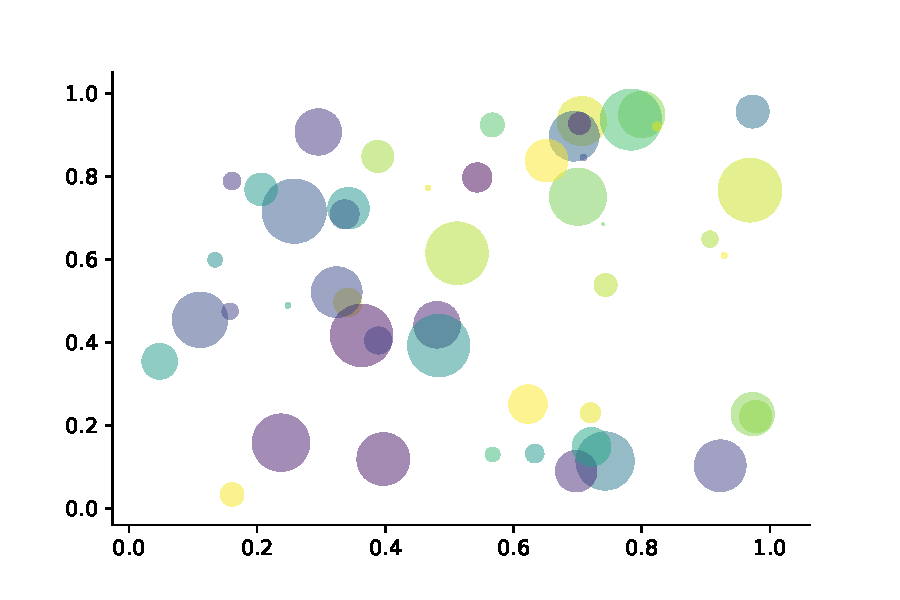
\includegraphics[width=0.6\textwidth]{scatter.pdf}
  \caption{散点图示例 $\hat{y}=a+bx$ \label{fig:scatter}}
\end{figure}

以最简单的一元线性模型来解释最小二乘法。什么是一元线性模型呢?监督学习中,如果预测的变量是离散的,我们称其为分类(如决策树,支持向量机等),如果预测的变量是连续的,我们称其为回归。回归分析中,如果只包括一个自变量和一个因变量,且二者的关系可用一条直线近似表示,这种回归分析称为一元线性回归分析。如果回归分析中包括两个或两个以上的自变量,且因变量和自变量之间是线性关系,则称为多元线性回归分析。对于二维空间线性是一条直线;对于三维空间线性是一个平面,对于多维空间线性是一个超平面。

\begin{property}\label{property:cauchy}
柯西列的性质
\begin{enumerate}
\item $\{x_k\}$ 是柯西列,则其子列 $\{x_k^i\}$ 也是柯西列。
\item $x_k\in \mathcal{R}^n$,$\rho(x,y)$ 是欧几里得空间,则柯西列收敛,$(\mathcal{R}^n,\rho)$ 空间是完备的。
\end{enumerate}
\end{property}

\begin{conclusion}
回归分析(regression analysis) 是确定两种或两种以上变量间相互依赖的定量关系的一种统计分析方法。运用十分广泛,回归分析按照涉及的变量的多少,分为一元回归和多元回归分析;按照因变量的多少,可分为简单回归分析和多重回归分析;按照自变量和因变量之间的关系类型,可分为线性回归分析和非线性回归分析。
\end{conclusion}

\begin{problemset}
\item 设 $A$ 为数域 $K$ 上的 $n$ 级矩阵。证明:如果 $K^n$ 中任意非零列向量都是 $A$ 的特征向量,则 $A$ 一定是数量矩阵。
\item 证明:不为零矩阵的幂零矩阵不能对角化。
\item 设 $A = (a_{ij})$ 是数域 $K$ 上的一个 $n$ 级上三角矩阵,证明:如果 $a_{11} = a_{22} = \cdots = a_{nn}$,并且至少有一个 $a_{kl} \not = 0 (k < l)$,则 $A$ 一定不能对角化。
\end{problemset}

\nocite{*}
\printbibliography
\appendix

\end{document}
